\documentclass{acm_proc_article-sp}

\usepackage[utf8]{inputenc}
\usepackage[T1]{fontenc}

\usepackage[activate=compatibility]{microtype}

% autoref command
\usepackage[pdftex,urlcolor=black,colorlinks=true,linkcolor=black,citecolor=black]{hyperref}
\def\sectionautorefname{Section}
\def\subsectionautorefname{Subsection}
\def\subfloatautorefname{Subfigure}

\usepackage[lofdepth,lotdepth]{subfig}

\usepackage{enumitem}

\usepackage{mathtools}

\usepackage{eurosym}

% give emph a normal fontsize
\let\oldemph\emph
\renewcommand{\emph}[1]{\oldemph{\fontsize{9}{9}\selectfont #1}}

% more readable footnote layout
\renewcommand{\footnotesize}{\fontsize{8pt}{10pt}}
\setlength{\footnotesep}{.5cm}

% todo macro
\usepackage{color}
\newcommand{\todo}[1]{\noindent\textcolor{red}{{\bf \{TODO}: #1{\bf \}}}}
\newenvironment{Todo}{\color{red}{\par{\bf TODO}}\everypar={\color{red}}{}}{}

% listings and Verbatim environment
\usepackage{fancyvrb}
\usepackage{relsize}
\usepackage{listings}
\usepackage{verbatim}
\newcommand{\defaultlistingsize}{\fontsize{8pt}{9.5pt}}
\newcommand{\inlinelistingsize}{\fontsize{8pt}{11pt}}
\newcommand{\smalllistingsize}{\fontsize{7.5pt}{9.5pt}}
\newcommand{\listingsize}{\defaultlistingsize}
\RecustomVerbatimCommand{\Verb}{Verb}{fontsize=\inlinelistingsize}
\RecustomVerbatimEnvironment{Verbatim}{Verbatim}{fontsize=\defaultlistingsize}
\lstset{frame=lines,captionpos=b,numberbychapter=false,escapechar=§,
        aboveskip=0.5em,belowskip=0em,abovecaptionskip=0em,belowcaptionskip=0em,
framexbottommargin=-1em,
        basicstyle=\ttfamily\listingsize\selectfont}

% use Courier from this point onward
\let\oldttdefault\ttdefault
\renewcommand{\ttdefault}{pcr}
\let\oldurl\url
\renewcommand{\url}[1]{\inlinelistingsize\oldurl{#1}}

% superscript for 1st, 2nd, etc.
\newcommand{\superscript}[1]{\ensuremath{^{\textrm{#1}}}}
%\newcommand{\subscript}[1]{\ensuremath{_{\textrm{#1}}}}
%\newcommand{\th}[0]{\superscript{th}}
%\newcommand{\st}[0]{\superscript{st}}
%\newcommand{\nd}[0]{\superscript{nd}}
%\newcommand{\rd}[0]{\superscript{rd}}

% linewrap symbol
\definecolor{grey}{RGB}{130,130,130}
\newcommand{\linewrap}{\raisebox{-.6ex}{\textcolor{grey}{$\hookleftarrow$}}}

% more pleasing quote environment
\usepackage{tikz}
\newcommand*{\openquote}{\tikz[remember picture,overlay,xshift=-7pt,yshift=1pt]
     \node (OQ) {\fontfamily{fxl}\fontsize{16}{16}\selectfont``};\kern0pt}
\newcommand*{\closequote}{\tikz[remember picture,overlay,xshift=2pt,yshift=-4.5pt]
     \node (CQ) {\fontfamily{fxl}\fontsize{16}{16}\selectfont''};}
\renewenvironment{quote}%
{\setlength{\parindent}{1cm}\par\openquote}
{\closequote\vspace{-4.5pt}
}

\makeatletter
\let\@copyrightspace\relax
\makeatother

\begin{document}

\title{Getting the Bigger Picture -- Extracting Media Items Covering Events from Multiple Social Networks}

\numberofauthors{3}
\author{
\alignauthor
\textbf{Thomas Steiner}\\
	\affaddr{Univ. Polit\`{e}cnica de Catalunya}\\
	\affaddr{Department LSI}\\
	\affaddr{08034 Barcelona, Spain,}\\
	\affaddr{tsteiner@lsi.upc.edu}
\alignauthor
\textbf{Raphaël Troncy}\\
	\affaddr{EURECOM}\\
	\affaddr{06560 Sophia Antipolis}\\
	\affaddr{France}\\
	\affaddr{rtroncy@eurecom.fr}
\and
\alignauthor
\textbf{Ruben Verborgh}\\ 	
	\affaddr{Ghent University -- IBBT, ELIS}\\
	\affaddr{Multimedia Lab}\\
	\affaddr{9050 Ghent, Belgium}\\
	\affaddr{ruben.verborgh@ugent.be}
\alignauthor
\textbf{Joaquim Gabarro}\\
	\affaddr{Univ. Polit\`{e}cnica de Catalunya}\\
	\affaddr{Department LSI}\\
	\affaddr{08034 Barcelona, Spain,}\\
	\affaddr{gabarro@lsi.upc.edu}
\alignauthor
\textbf{Rik Van de Walle}\\
	\affaddr{Ghent University -- IBBT, ELIS}\\
	\affaddr{Multimedia Lab}\\
	\affaddr{9050 Ghent, Belgium}\\
	\affaddr{rik.vandewalle@ugent.be}
}

\maketitle

\begin{abstract}
\todo{
Core contributions:
Social network and media platform agnostic media item search, and search results alignment.
Search results semantic enrichment by putting microposts and media items in relation.
Cross-channel popularity analysis.
Visual clustering, photos contained in videos.
}
\end{abstract}

\category{H.3.4}{Information Systems}{Information Storage and Retrieval}[World Wide Web]
\category{H.3.5}{Online Information Services}{Web-based services}

\keywords{\todo{Keywords}}

% Responsible: Raphaël
\section{Introduction} \label{sec:introduction}
\todo{
Say what we do, and what we don't.
Say that we are not competing with the TRECVID guys, as they have all the data, and we have to get it first.
}

\subsection{Used Terms}
In this Subsection, we provide necessary definition for the terms that we will use throughout this paper.

\begin{description}
\item[Social Network]
A \emph{social network} is an online service or \emph{media platform} that focuses on building and reflecting of social relations among people, who, for example, share interests and/or activities.
The boundary between social networks and media platforms is fluid.
There are media platforms where people can upload their content with optionally content viewers -- in a relation to the original uploader or not -- having the possibility to react in form of comments, or in form of likes or dislikes.
An example is YouTube.
There are social networks where people can update their status, post links to stories, or upload their content with necessarily viewers -- standing in a relation or not -- having the option to react.
An example is Facebook.
Finally, there are hybrid forms, where social networks -- typically via third party applications -- integrate with media platforms.
An example is the TweetDeck for Twitter application and their integration with TwitPic.

\item[Media Item]
A \emph{media item} in the context of this paper is any video or image file that gets distributed via a social network. An example can be a baby photo that someone shares on Facebook. 

\item[Micropost]
A \emph{micropost} is any textual status update that can -- but not has to -- accompany a media item. An example can be a status update accompanying the previously mentioned baby photo saying ``life is full of wonders, and you are one of them''.

\item[Event]
An \emph{event} is an observable occurrence, phenomenon or an extraordinary occurrence with not necessarily defined start and/or end points. An event with a defined start (May 15, 2011), however, no concrete end, are the 2011 protests in Spain. An event with both start and end can be a concert.
\end{description}

% Responsible: Thomas
\section{Social Networks \& Media Items}

\subsection{Media Item Extraction}
\todo{
Talk about media item recall (ratio items that match the query vs. items that match the query with media items).
}

\subsection{API Access vs. Web Scraping}
An \emph{Application Programming Interface (API)} in the sense of Web-based API is a programmatic specification intended to be used as an interface by software components on client and server to communicate with each other.

\emph{Web scraping} is the process of automatically extracting information from websites.
Web scraping involves practical solutions based on existing technologies that are often entirely ad hoc.
Examples of such technologies are regular expressions or DOM parsing of Web pages into a DOM tree.

The difference to the somewhat related concept of \emph{screen scraping} is that screen scraping relies on the visual layout of a website, whereas Web scraping relies on the textual and/or hierarchical structure of websites.

Social networks today are very much perceived as ``walled gardens'', excellently illustrated by a cartoon by David Simonds~(\autoref{fig:DavidSimonds}).
As with Orwell, where some animals are more equal than others, some social networks are more walled than others.
Some social networks have full read and write access via specified APIs.
An example is Twitter.
Other social networks have read access via APIs.
An example is Google+.
Interestingly, some media platforms have just write API support, however, no read support, which requires us to fall back to Web scraping the website in order to retrieve data.
An example is Img.ly.

\begin{figure}
\centering
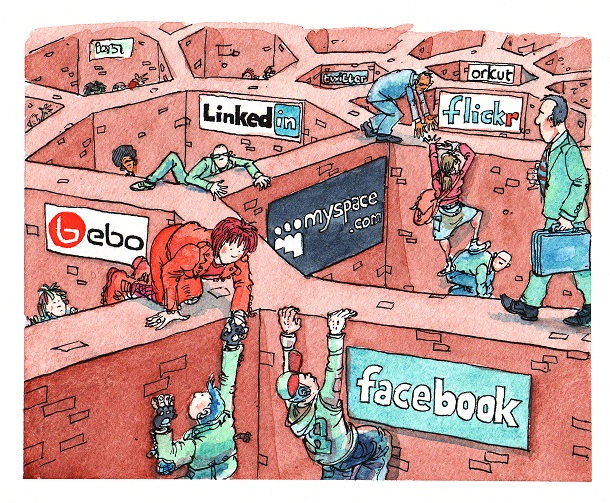
\includegraphics[width=1.0\linewidth,trim=16px 17px 12px 15px,clip]{./resources/davidsimonds.jpg}
\caption{David Simonds illustrates social networks as walled gardens due to their (by design) lock-in effects~\cite{DavidSimonds}.}
\label{fig:DavidSimonds}
\end{figure}

% Responsible: Thomas
\section{Implementation Details}
In this Section, first, we introduce the common data format used consistently between all considered social networks,
second, we explain the architecture for different kinds of media item collectors,
and third, show the steps in the media item processing chain.

\subsection{Data Format}
Our approach being agnostic of concrete social networks, we offer a common alignment schema for all considered social networks, which allows us to treat each social network's data the same way.
The resulting set of metadata for a media item can be seen below:
\begin{itemize}
  \item	\textbf{Media URL}, the deep link to the media item, e.g., \url{http://farm7.staticflickr.com/6059/6290784192_567346ba6a_o.jpg}.
  \item \textbf{Type}, the type of the media item, one out of ``photo'' or ``video''.
  \item \textbf{Story URL}, the URL of the micropost where the media item appeared, e.g., \url{http://www.flickr.com/photos/96628098@N00/6290784192/}.
  \item \textbf{Message}, the concrete micropost or description text in raw format, e.g., ``Laura. \#lumixg20f17, \#iswc2011, \#internationalsemanticwebconference, \#bonn, \#germany''.
  \item \textbf{Clean}, the concrete cleaned micropost or description text with some characters (e.g., hash sign) removed, e.g., ``Laura. lumixg20f17, iswc2011, internationalsemanticwebconference, bonn, germany''.
  \item \textbf{User}, the URL of the author of the micropost, e.g., \url{http://www.flickr.com/photos/96628098@N00/}.
  \item \textbf{Published}, the timestamp of when the micropost was authored, or the media item was uploaded, e.g., \texttt{2011\-10\-27T12:24:41Z}.
\end{itemize}
\autoref{lst:media} shows the sample output of a media collector for the Google+ media provider.


% Use a consistent example from one of the experiments
\begin{lstlisting}[caption={Sample output of the media collector showing a Facebook post processed with named entity extraction and disambiguation (slightly edited for legibility).},label={lst:media}]
{
  "Facebook": [
    {
      "mediaurl": "http://video.ak.fbcdn.net/...",
      "storyurl": "https://www.facebook.com/perma-
          link.php?story_fbid=231781590231029&id=
          1254772464",
      "message": {
        "text": "Videoed between Hamburg and Sny-
            der.. Thought I would share.",
        "clean": "Videoed between Hamburg and Sny
            der.. Thought I would share.",
        "entities": [
          [
            {
              "name": "Hamburg",
              "relevance": 0.82274,
              "uri": "http://dbpedia.org/resource/
                  Hamburg"
            },
            {
              "name": "Snyder",
              "relevance": 0.857,
              "uri": "http://dbpedia.org/resource/
                  Snyder,_Texas"
            }
          ]
        ]
      },
      "user": "https://www.facebook.com/
          profile.php?id=1254772464",
      "type": "video",
      "timestamp": 1326371479000,
      "published": "2012-01-12T12:31:19Z"
    }
  ]
}
\end{lstlisting}

\subsection{Media Item Collectors}
In the context of this paper, we have developed media item collectors for the social networks Google+, MySpace, Facebook, Twitter, Instagram, YouTube, and Flickr,
with additional support for the media platforms img.ly, yfrog, MobyPicture, and TwitPic.
As can be seen in \autoref{fig:architecture},
due to the lack of search APIs on some of the involved services,
we were forced to a two-fold approach that involves Web scraping alongside regular API calls.

\begin{figure*}
\centering
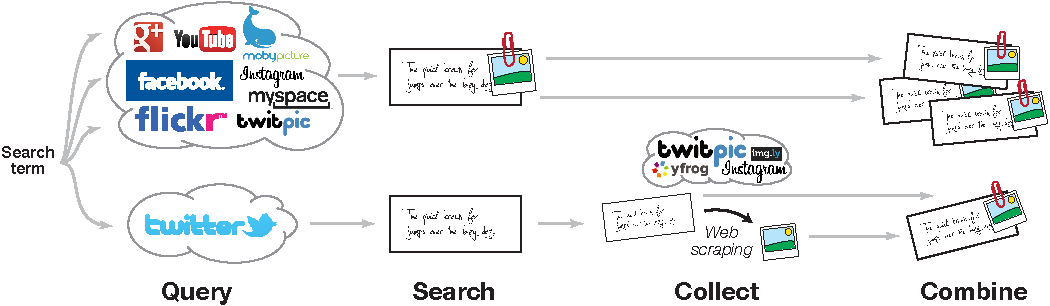
\includegraphics[width=1.0\linewidth]{./resources/architecture.pdf}
\caption{The media item collector architectural overview shows the hybrid approach to the media item extraction process using a combination of API access and Web scraping.}
\label{fig:architecture}
\end{figure*}

\subsection{Media Item Processing}

\subsubsection{Machine Translation}

\subsubsection{Part of Speech Tagging}
% Maybe remove this?

\subsubsection{Named Entity Disambiguation}

\subsubsection{Irrelevant Media Item Pruning}
\todo{
De-duplication of photos and videos.
Detection of photos contained in videos.
This is not about visual relevance checks => point to related work
}

\section{Experiments}
\label{sec:experiments}
% Responsible: Thomas
For our experiments, we have taken into account several events that happened in the period of January 10 to 19, 2012, and thus were the subject of discussion on various social networks.
We have captured event-related media items and microposts, and made the data available online\footnote{Event-related media items and microposts: \url{http://www.lsi.upc.edu/~tsteiner/experiments/icmr2012/}}. 

\subsection{Considered Events}
In this Subsection, we give an objective and short overview on the context of the considered events in order to give the reader the necessary background knowledge.
% Add to each event some categorization: political, technical,…
% Add to each event the duration with start and end if possible.

\paragraph{SOPA Blackout}
The Stop Online Piracy Act (SOPA) is a bill of the United States proposed in 2011 to fight online trafficking in copyrighted intellectual property and counterfeit goods.
On January 18, English Wikipedia, Reddit, and several other Internet companies coordinated a service blackout to protest SOPA and its sister bill, the Protect IP Act.
Other companies, including Google, posted links and images in an effort to raise awareness\footnote{SOPA Blackout: \url{http://sopablackout.org/learnmore/}}.

\paragraph{Assad Speech}
On January 10, 2012, Syrian President Bashar al-Assad delivered a lengthy televised talk strongly defending his government's actions and motivations, despite world pressure on his embattled government for its 10-month crackdown on protesters\footnote{Assad Speech: \url{http://www.cnn.com/2012/01/10/world/meast/syria-unrest/}}. 

\paragraph{Christian Wulff Case}
Since December 2011, German President Christian Wulff faces controversy over discrepancies in statements about a loan while governor of Lower Saxony.
When the affair settled down, it was revealed that he had applied pressure on Springer Press to delay revelations on the issue until he was back from a visit abroad.
When Wulff found out that a tabloid was going to break the story, he left a message on the voice mail of the editor-in-chief in which he threatened to take legal action\footnote{Christian Wulff Case: \url{http://www.spiegel.de/international/germany/0,1518,804631,00.html}}.

\paragraph{Dixville Notch}
Dixville Notch is an unincorporated village in Dixville township of Coos County, New Hampshire, USA, best known in connection with its longstanding middle-of-the-night vote in the U.S. presidential election.
In a tradition that started in the 1960 election, all the eligible voters in Dixville Notch gather at midnight in the ballroom of The Balsams.
This year, on January 10, 2012, the voters cast their ballots and the polls officially closed one minute later\footnote{Dixville Notch: \url{http://www.washingtonpost.com/2012/01/09/gIQANslKnP_story.html}}.

\paragraph{Free Mobile Launch}
Free Mobile is a French mobile broadband company, part of the Iliad group.
On January 10, 2012, a long-awaited mobile phone package for \EUR{19.99} with calls included to 40 countries, texts, multimedia messages and Internet was announced by the Iliad group's Chief Strategy Officer, Xavier Niel\footnote{Free Mobile Launch: \url{http://www.nytimes.com/2012/01/11/technology/iliad-takes-aim-at-top-mobile-operators-in-france.html}}.

\paragraph{Costa Concordia Disaster}
The Costa Concordia is an Italian cruise ship that hit a reef and partially sank on January 13, 2012 off the Italian coast.
The vessel ran aground at Isola del Giglio, Tuscany, resulting in the evacuation of 4,211 people on board\footnote{Coosta Concordia Disaster: \url{http://www.costacruise.com/B2C/USA/Info/concordia_statement.htm}}.

\paragraph{CES Las Vegas}
The International Consumer Electronics Show (CES) is a major technology-related trade show held each January in the Las Vegas Convention Center.
Not open to the public, the Consumer Electronics Association-sponsored show typically hosts previews of products and new product announcements\footnote{CES Las Vegas: \url{http://www.cesweb.org/aboutcea.asp}}.

\paragraph{Cut the Rope Launch}
% Sub-event of CES Las Vegas
On January 10, 2012 during Microsoft's keynote at CES, the HTML5 version of the popular mobile game \textit{Cut the Rope} was announced\footnote{Cut the Rope Launch: \url{http://ces.cnet.com/8301-33377_1-57356403/}}.

\paragraph{Ubuntu TV Launch}
% Sub-event of CES Las Vegas
Ubuntu TV by Canonical, based on the user interface Unity, is a variant of the Ubuntu operating system, designed to be a Linux distribution specially adapted for embedded systems in televisions. It was announced by Canonical on January 10, 2012, at CES\footnote{Ubuntu TV: \url{http://www.theverge.com/2012/1/9/2695387/ubuntu-tv-video-hands-on}}.

\subsection{Dataset}
\label{subsec:dataset}
During the examination of our dataset, we observed that the process of image de-duplication is by no means a solved issue.
Content-based image retrieval (CBIR) uses features like color, texture, and shape to search images from large-scale databases.
The same technique, however, can also be used for the de-duplication of photographs~\cite{Pattabhi2011}.
We used a CBIR-based image duplication detection software\footnote{PhotoSweeper: \url{http://itunes.apple.com/us/app/photosweeper/id463362050?mt=12}} that allows for manual algorithm and threshold selection to detect duplicates in the dataset.
For each considered event, we manually selected the best settings to limit the number of duplicate misses and false positives.
The main problem with the dataset is its diversity.
It ranges from entirely sharp screenshots in all sorts of formats (e.g., for the SOPA Blackout), to blurry cell phone images in standard photo formats (e.g., for the Free Mobile Launch).
A common performance tweak to speed up the duplication detection process is to shrink images to quadratic bitmaps.
In the context of our dataset, however, this approach is counterproductive, as a screenshot of a rectangular IAB $728 \times 90$ ``leaderboard'' banner is treated the same as a standard 3.1 megapixels ($2048 \times 1536$) cell phone photo.
In practice, this led to many incorrect results, requiring manual de-duplication with some events.
Our data set contained 448 images in total, with the average file size being $\sim$0.7MB (314.5MB in total).

\begin{table*}[htbp]
  \begin{tabular}{ | c | c | c | }
    \hline
    \textbf{Social Network} & \textbf{Images} & \textbf{Videos}\\
    \hline
    Google+ & 3 & 2\\
    MySpace & 0 & 0\\
    Facebook & 0 & 0\\
    Twitter & 2 & 0\\
    Instagram & 0 & 0\\
    YouTube & 0 & 10\\
    Flickr & 10 & 0\\
    MobyPicture & 0 & 0\\
    TwitPic & 0 & 0\\
    \hline
  \end{tabular}
  \label{tab:assad}
  \caption{\textbf{Assad Speech} -- Network Distribution. \textbf{Total images:} 15. \textbf{Total videos:} 12.}
\end{table*}

\begin{table*}[htbp]
  \begin{tabular}{ | c | c | c | }
    \hline
    \textbf{Social Network} & \textbf{Images} & \textbf{Videos}\\
    \hline
    Google+ & 5 & 0\\
    MySpace & 0 & 0\\
    Facebook & 0 & 2\\
    Twitter & 5 & 0\\
    Instagram & 20 & 0\\
    YouTube & 0 & 10\\
    Flickr & 10 & 0\\
    MobyPicture & 1 & 0\\
    TwitPic & 19 & 0\\
    \hline
  \end{tabular}
  \label{tab:sopa}
  \caption{\textbf{Blackout SOPA} -- Network Distribution. \textbf{Total images:} 60. \textbf{Total videos:} 12.}
\end{table*}

\begin{table*}[htbp]
  \begin{tabular}{ | c | c | c | }
    \hline
    \textbf{Social Network} & \textbf{Images} & \textbf{Videos}\\
    \hline
    Google+ & 5 & 3\\
    MySpace & 0 & 0\\
    Facebook & 0 & 1\\
    Twitter & 2 & 0\\
    Instagram & 20 & 0\\
    YouTube & 0 & 10\\
    Flickr & 10 & 6\\
    MobyPicture & 1 & 0\\
    TwitPic & 20 & 0\\
    \hline
  \end{tabular}
  \label{tab:ces}
  \caption{\textbf{CES Las Vegas} -- Network Distribution. \textbf{Total images:} 58. \textbf{Total videos:} 20.}
\end{table*}

\begin{table*}[htbp]
  \begin{tabular}{ | c | c | c | }
    \hline
    \textbf{Social Network} & \textbf{Images} & \textbf{Videos}\\
    \hline
    Google+ & 7 & 0\\
    MySpace & 8 & 0\\
    Facebook & 0 & 0\\
    Twitter & 2 & 0\\
    Instagram & 2 & 0\\
    YouTube & 0 & 10\\
    Flickr & 10 & 2\\
    MobyPicture & 3 & 0\\
    TwitPic & 20 & 0\\
    \hline
  \end{tabular}
  \label{tab:wulff}
  \caption{\textbf{Christian Wulff Case} -- Network Distribution. \textbf{Total images:} 52. \textbf{Total videos:} 12.}
\end{table*}

\begin{table*}[htbp]
  \begin{tabular}{ | c | c | c | }
    \hline
    \textbf{Social Network} & \textbf{Images} & \textbf{Videos}\\
    \hline
    Google+ & 15 & 1\\
    MySpace & 10 & 0\\
    Facebook & 0 & 1\\
    Twitter & 3 & 0\\
    Instagram & 20 & 0\\
    YouTube & 0 & 10\\
    Flickr & 10 & 10\\
    MobyPicture & 4 & 0\\
    TwitPic & 18 & 0\\
    \hline
  \end{tabular}
  \label{tab:concordia}
  \caption{\textbf{Costa Concordia Disaster} -- Network Distribution. \textbf{Total images:} 80. \textbf{Total videos:} 22.}
\end{table*}

\begin{table*}[htbp]
  \begin{tabular}{ | c | c | c | }
    \hline
    \textbf{Social Network} & \textbf{Images} & \textbf{Videos}\\
    \hline
    Google+ & 5 & 1\\
    MySpace & 6 & 0\\
    Facebook & 0 & 0\\
    Twitter & 4 & 0\\
    Instagram & 20 & 0\\
    YouTube & 0 & 10\\
    Flickr & 10 & 10\\ 
    MobyPicture & 20 & 0\\
    TwitPic & 20 & 0\\
    \hline
  \end{tabular}
  \label{tab:rope}
  \caption{\textbf{Cut the Rope Launch} -- Network Distribution. \textbf{Total images:} 85. \textbf{Total videos:} 21.}
\end{table*}

\begin{table*}[htbp]
  \begin{tabular}{ | c | c | c | }
    \hline
    \textbf{Social Network} & \textbf{Images} & \textbf{Videos}\\
    \hline
    Google+ & 4 & 1\\
    MySpace & 9 & 0\\
    Facebook & 0 & 0\\
    Twitter & 3 & 0\\
    Instagram & 0 & 0\\
    YouTube & 0 & 3\\
    Flickr & 10 & 10\\ 
    MobyPicture & 0 & 0\\
    TwitPic & 1 & 0\\
    \hline
  \end{tabular}
  \label{tab:dixville}
  \caption{\textbf{Dixville Notch} -- Network Distribution. \textbf{Total images:} 27. \textbf{Total videos:} 14.}
\end{table*}

\begin{table*}[htbp]
  \begin{tabular}{ | c | c | c | }
    \hline
    \textbf{Social Network} & \textbf{Images} & \textbf{Videos}\\
    \hline
    Google+ & 6 & 0\\
    MySpace & 1 & 0\\
    Facebook & 0 & 0\\
    Twitter & 2 & 0\\
    Instagram & 20 & 0\\
    YouTube & 0 & 10\\
    Flickr & 10 & 0\\ 
    MobyPicture & 2 & 0\\
    TwitPic & 20 & 0\\
    \hline
  \end{tabular}
  \label{tab:freemobile}
  \caption{\textbf{Free Mobile Launch} -- Network Distribution. \textbf{Total images:} 61. \textbf{Total videos:} 10.}
\end{table*}

\begin{table*}[htbp]
  \begin{tabular}{ | c | c | c | }
    \hline
    \textbf{Social Network} & \textbf{Images} & \textbf{Videos}\\
    \hline
    Google+ & 6 & 1\\
    MySpace & 0 & 0\\
    Facebook & 0 & 0\\
    Twitter & 0 & 0\\
    Instagram & 0 & 0\\
    YouTube & 0 & 10\\
    Flickr & 10 & 9\\ 
    MobyPicture & 2 & 0\\
    TwitPic & 2 & 0\\
    \hline
  \end{tabular}
  \label{tab:ubuntutv}
  \caption{\textbf{Ubuntu TV Launch} -- Network Distribution. \textbf{Total images:} 20. \textbf{Total videos:} 20.}
\end{table*}

\begin{Todo}
Table with pure stats about
- number of total media items
- number of unique media items
- network distribution of media items 
- named entities

\end{Todo}

\subsection{Results}
\todo{
- Visual gallery
- What can we say about each event (networks, diversity,…)
}

\subsection{Discussion}
% Ranking factors:
% Popularity [ReTweets, Likes, +1s, number of views, presence on networks]
% User diversity [more media from more different users]
% Media item diversity [more media that looks different]
% Representation: feature more popular items bigger(?), or longer(?)

% Responsible: Ruben
\section{Related Work} \label{sec:relatedwork}
% Separate related work in fields:
% - media item collection from social networks
% - event summarization

% Highlight what Twitter is doing (most popular image/video)
% Google news top stories
% Automatic gallery creation

\begin{comment}
\cite{Fabro2012}
Just Flickr and YouTube.
Use clustering algorithm for textual content.
Duplicate detection via Color and Edge Directivity Descriptor (CEDD).
Restrict selection to geolocated content and time period.
\end{comment}

\begin{comment}
\cite{Liu2011}
Objective is to aggregate heterogeneous event information sources using Linked Data principles.
Just Flickr and YouTube, with additional media from event information sources.
Query with "what", "where", "when", uses "title"+"time" and "geotag"+"time".
Use machine-tagged media items to find visually similar media items.
\end{comment}

A~first category of related work includes research that aims to collect, align, and organize media for trends or events.
Liu \emph{et al.} combine semantic inferencing and visual analysis to automatically find media to illustrate events~\cite{Liu2011}.
They interlink large datasets of event metadata and media with the Linking Open Data Cloud~\cite{LODcloud}.
Approaches for alignment use visual, temporal, and spacial similarity measures to map multiple photo streams of the same events~\cite{Yang2011}.
Other ways to collect and order media from social networks use user-driven metadata such as geospatial information~\cite{Crandall}.

Another relevant work area is duplicate and near-duplicate media detection.
As evident from several experiments and mentioned in \autoref{subsec:dataset},
providing unique media content to users is still an unsolved problem.
Work on ordinal measures for image correspondence started in the last decade of the 20\superscript{th}~century~\cite{Bhat}.
Recently, Chum \emph{et al.} have proposed a near-duplicate image detection method using MinHash and tf--idf weighting~\cite{Chum}.
A~method for both images and video has been proposed by Yang \emph{et al.}~\cite{Yang}.
Specialized methods for video exist as well~\cite{Min, Wu}, an excellent survey of which has been conducted by Lian \emph{et al.}~\cite{Lian}.

When unique media items have been collected, the remaining task is to summarize events by selecting the most relevant media fragments.
An article by Fabro and B\"osz\"orm\'enyi~\cite{Fabro2012} details the summarization and presentation of events from content retrieved from social media.
Nowadays, many domain-specific methods already exhibit good accuracy, for example in the sports domain~\cite{Li1,Li2}.
However, the challenge in this field is to find methods that are content-agnostic.
Methods that exploit semantic information~(\emph{e.g.}, \cite{Chen}) will likely provide high-quality results in the future,
but today's most relevant summaries are produced by user interaction~\cite{Olsen}.

% Temporarily added to simplify writing and reading Future Work section
\clearpage

\section{Conclusion and Future Work}
% Conclusion
\todo{Write conclusion}

% Future work
% Responsible: Ruben
In this work, the focus has been on extracting visual media and associated textual messages from social networks.
One possibility for future work would therefore be to pursue our efforts in this direction by supporting more social networks and improving our Web scrapers.
This could significantly improve the quantity and diversity of considered media and messages,
given the fact that different kinds of information are shared to different networks~\cite{ConsumersLook}.

A~more innovative direction, however, is to incorporate techniques from multimedia analysis into the process,
as this will create a~multi-modal environment where different factors are used to organize social content.
This can start with context-independent analyses, such as the content deduplication techniques discussed in \autoref{sec:relatedwork},
or visual quality metrics~(sharpness, contrast\ldots) to display original and high-quality media more prominent in results.
Furthermore, this identification of original content can allow users to choose a~balance between popularity~(favor omnipresent content) and originality~(promote rare content).

Much more potential, however, is expected to reside in context-aware multimedia analysis,
since many media items contain a~message that is complementary to the text.
For example, facial detection~\cite{ViolaJones} and eventually recognition~\cite{Wright}
can signify the presence of specific people in a~media fragment.
As visual recognition systems grow more powerful, more objects will eventually be recognizable by machines~\cite{Serre},
which would allow generating \emph{visual hashtags} that describe the content \emph{inside} of the media item.
This would positively influence the diversity of automated summarizations.

It remains important, however, to view the media and the associated text as a~whole,
since the text could convey a~sentiment about or an~explanation of the visual data.
Using named entity recognition~\cite{NERD}, the important semantic elements in the message text can be identified to build an understanding of its meaning.
The contents of the message could subsequently be used to narrow down the search space for visual factors, enabling cross-fertilization between the textual and visual analysis, which results in effective, context-aware analysis possibilities~\cite{verborgh_mtap_2011}.

\section*{Acknowledgments}
The research activities as described in this paper were funded by Ghent University, the Interdisciplinary Institute for Broadband Technology (IBBT), the Institute for the Promotion of Innovation by Science and Technology in Flanders (IWT), the Fund for Scientific Research Flanders (FWO Flanders), and the European Union.

This work was partially supported by the European Commission under Grant No. 248296 FP7 \mbox{I-SEARCH} project.
Joaquim Gabarr\'o is partially supported by TIN-2007-66523 (FORMALISM), and SGR 2009-2015 (\mbox{ALBCOM}).

% back to normal size Computer Modern for URLs in bibliography
\let\ttdefault\oldttdefault
\let\url\oldurl

\bibliographystyle{abbrv}
\bibliography{icmr2012}

\balancecolumns
\end{document}